% Created 2018-06-06 Wed 20:51
% Intended LaTeX compiler: pdflatex
\documentclass[10pt,a4paper]{article}
\usepackage[utf8]{inputenc}
\usepackage[T1]{fontenc}
\usepackage{graphicx}
\usepackage{grffile}
\usepackage{longtable}
\usepackage{wrapfig}
\usepackage{rotating}
\usepackage[normalem]{ulem}
\usepackage{amsmath}
\usepackage{textcomp}
\usepackage{amssymb}
\usepackage{capt-of}
\usepackage{hyperref}
\usepackage[utf8]{inputenc}
\usepackage[T1]{fontenc}
\usepackage{amssymb}
\usepackage{amsmath}
\usepackage{amsfonts}
\usepackage{setspace}
\usepackage{lipsum}
\usepackage{textcomp}
\usepackage{float}
\usepackage{graphicx}
\usepackage{array}
\usepackage{listings}
\usepackage{color}
\usepackage{tcolorbox}
\usepackage{bm}
\usepackage{matlab-prettifier}
\usepackage[margin=3cm]{geometry}
\usepackage[titletoc,title]{appendix}
\setlength{\parskip}{1.1ex}
\setlength{\parindent}{0ex}
\author{Yuchen Zhou}
\date{\today}
\title{}
\hypersetup{
 pdfauthor={Yuchen Zhou},
 pdftitle={},
 pdfkeywords={},
 pdfsubject={},
 pdfcreator={Emacs 25.2.1 (Org mode 9.1.1)}, 
 pdflang={English}}
\begin{document}

\begin{titlepage}
	\newcommand{\HRule}{\rule{\linewidth}{0.5mm}} % change thickness
	
	\center % Centre everything on the page
	
	%------------------------------------------------
	%	Headings
	%------------------------------------------------
	
	\textsc{\LARGE University of Cambridge}\\[0.4cm]
	\textsc{\LARGE Engineering Tripos Part IIA}\\[1.5cm]
	
	%------------------------------------------------
	%	Title
	%------------------------------------------------
	
	\HRule\\[0.4cm]
	
  \begin{center}
    \setstretch{0.8}
    \huge\bfseries GF2: Software\\[0.8cm]
  \end{center}

	{\LARGE\bfseries Final Report}\\[0.4cm] % Title of your document
	
	\HRule\\[1.5cm]
	
	%------------------------------------------------
	%	Author(s)
	%------------------------------------------------
	
	%\begin{minipage}{0.4\textwidth}
	%	\begin{flushleft}
	%		\large
	%		\textit{Author}\\
	%		Yuchen \textsc{Zhou}\\ % Your name
  %    \texttt{yz493@cam.ac.uk} % Your email
	%	\end{flushleft}
	%\end{minipage}
	%~
	%\begin{minipage}{0.4\textwidth}
	%	\begin{flushright}
	%		\large
	%		\textit{Supervisor}\\
	%		Dr. Richard \textsc{Roebuck}\\ % Supervisor's name
  %    \texttt{rlr20@hermes.cam.ac.uk} % Supervisor's email
	%	\end{flushright}
	%\end{minipage}
	
	% If you don't want a supervisor, uncomment the two lines below and comment the code above
	%{\large\textit{Author}}\\
  {\Large
	  Yuchen \textsc{Zhou}\\ % Your name
    Magdalene College\\
    Team 4\\[1.5cm]
    Email: \texttt{yz493@cam.ac.uk}
  }

	
	%------------------------------------------------
	%	Date
	%------------------------------------------------
	
	\vfill\vfill % Position the date 3/4 down the remaining page
	
	{\large\today} % Date, change the \today to a set date if you want to be precise
	
	\vfill\vfill % Push the date up 1/4 of the remaining page

	%------------------------------------------------
	%	Abstract
	%------------------------------------------------

\end{titlepage}


\section{Introduction}
\label{sec:org4fc4869}

In the coursework assignment we have implemented linear and RBF
classifiers based on maximum likelihood estimation (MLE). A practical
problem of MLE classifiers is that they are likely to suffer from data
overfitting (high variance). In the FTR assignment we are going to
implement a \emph{Bayesian classifier} which includes a Gaussian prior to
penalise high variance of our model parameters. In order to obtain the
predictive distribution (which is an integration with respect to the
posterior distribution over all possible model parameters), \emph{Laplace
approximation} is used to obtain a Gaussian approximation of the
posterior distribution. In the hyperparameter tuning stage, we also
need to maximise the \emph{model evidence} to get the optimal model
hyperparameters. 

This report first goes through all the necessary theory involved in
the Bayesian classifier and then explains the core Python code used in
the classifier implementation. The final results are presented in
terms of predictive distribution contour plots, train/test
log-likelihoods and confusion matrices, which we will discuss
carefully in the end

\section{Functions of the Logic Simulator}
\label{sec:org6ac67bb}

As its name suggests, the logic simulator simply just simulates the
real-world logic circuits on computers. It can read logic circuit
configurations into the software from text definition files, construct
and simulate the circuits, and display the simulation results on the
screen. The following sub-sections contain detailed description of the
functions of the logic simulator, from different perspectives.

\subsection{Basic functions achievable through definition file statements}
\label{sec:orga772621}
\label{orgb2fd366}

A valid definition file consists of statements which specify all the
initial configurations of the user's logic circuit. Each statement
represents one of the three basic functions: define a list of devices
of a certain device type (DEVICE), connect two device ports together
(CONNECT), and monitor a list of device outputs (MONITOR). Each
statement should be enclosed by a single pair of parentheses.

\subsubsection{Device definition}
\label{sec:org99cb2bd}

A list of devices of a certain device type can be defined through a
statement of the following format:

\texttt{(DEVICE device1 device2 ... is/are device\_type [qualifier])}

where the available device types are briefly described as follows:
\begin{center}
\begin{tabular}{|c|c|c|c|c|}
\hline
Device type(s) & Inputs & Outputs & Has qualifier? & Qualifier description\\
\hline
CLOCK & 0 & 1 & Yes & Change state every n cycles\\
SWITCH & 0 & 1 & Yes & Initial state (set/clear)\\
AND NAND OR NOR & 1-16 & 1 & Yes & Number of inputs\\
DTYPE & 4 & 2 & No & \\
XOR & 2 & 1 & No & \\
RC & 0 & 1 & Yes & Output falls low after n cycles\\
NOT & 1 & 1 & No & \\
\hline
\end{tabular}
\end{center}

The device definition statement starts with the keyword \texttt{DEVICE},
followed by a list of device names (cannot be empty), the keyword \texttt{is}
or \texttt{are}, and the device type (and possibly a qualifier) at the end.
User must provide a valid qualifier for a device type that needs a
qualifier (e.g. \texttt{CLOCK}, \texttt{RC}) and should not give a qualifier if the
device type does not need one (e.g. \texttt{DTYPE}, \texttt{NOT}).

If the device definition statement is valid, logic simulator will add
the devices to the device list, and the ports of these devices can be
further connected or monitored. In addition, for the \texttt{SWITCH}
devices, their states (set/clear) can be changed after the simulation
starts.

\subsubsection{Connecting device ports}
\label{sec:orgaffd8c6}
\label{org6f6e406}

Two device ports can be connected together by a statement of the
following format:

\texttt{(CONNECT device\_port1 to device\_port2)}

The connection statement starts with the keyword \texttt{CONNECT}, followed
by two device ports with the keyword \texttt{to} in between. In general, the
format of the device port name should be \texttt{device\_name.port\_name}.
There is only one special case, where the user should directly use the
\texttt{device\_name} as the device port name when that device has only one
output port.

The connection statement would be valid only if one port is an input
and the other is an output. Also, an output can be connected to
multiple inputs, but an input can only be connected to one output.

\subsubsection{Monitoring device ports}
\label{sec:orgfb7a04d}

A list of device ports can be monitored by a statement of the
following format:

\texttt{(MONITOR device\_port1 device\_port2 ...)}

The monitor definition statement begins with the keyword \texttt{MONITOR},
followed by a list of device ports to be monitored. Each device port
name conforms to the format specified in Section \ref{org6f6e406}. In the
logic simulator, only device outputs are allowed to be monitored. The
waveforms of the monitored outputs will finally be displayed on the
screen.

\subsection{Definition file read-in and error report}
\label{sec:org38e6e0d}

When the user has a definition file ready, he/she can open that file
in the logic simulator by clicking \texttt{File->Open} and use the system's
default file browser (a pop-up window) to select the file. The logic
simulator will try to read and interpret the statements one by one,
and gradually build the circuit on the fly. If the definition file is
error-free, nothing will happen and the user can proceed by clicking
the \texttt{Run} button (this conforms to the Unix philosophy - `no news is
good news'). 

In case that the definition file contains errors, a detailed error
report will be shown in a pop-up window, with description and location
(line number and position in the line) of each error occured, in order
to provide useful information to the user so that he/she can locate
and correct the errors more easily. There are two main categories of
errors, namely \emph{syntactic error} and \emph{semantic error}. Syntactic
errors occur when parts of the definition file don't obey the grammar
as specified in the EBNF file (e.g. mistyping keywords), while
semantic errors occur when parts of the file are grammatically correct
but don't make any sense (e.g. connecting two inputs). After
correcting all the errors, the user can open the file again and
proceed with the simulation.

\subsection{Display of waveforms of the monitored device outputs}
\label{sec:orgf17cd14}

If the definition file read-in stage has been successful, the user can
enter a number in the textbox at the top of the main control panel to
specify the initial simulation cycles, and then click the \texttt{Run} button
below the textbox to start the simulation. The waveforms of the
monitored device outputs will then be displayed on the main canvas.

The waveforms of the monitored signals are drawn in the main canvas
from bottom to top, with a red ruler right below the waveforms which
indicates the number of simulation cycles. If the user moves cursor
into the canvas, a vertical cursor line will be shown to point the
current cycle number on the ruler, and a yellow hoverbox will appear
with information of current cycle number, port name and the output
value (high/low).

By our settings, the maximum number of simulation cycles per page is
fixed at 60. If more than 60 cycles are simulated, the user can use
the \texttt{Prev Page / Next Page} buttons or enter a page number and click
the \texttt{Goto} button to navigate among the pages. The waveforms can also
be zoomed in/out horizontally by using the two icons at the bottom of
the control panel, or place the cursor inside the canvas and use the
scroll wheel. In addition, each monitored signal can be moved up/down
by pressing and holding the left button and drag the signal
upward/downward.


\subsection{Modifications of circuit and simulator settings}
\label{sec:org38fd84f}

The user can modify some of the states of the simulator after
successfully parsing a definition file. For instance, the outputs of
the switches can be changed by selecting the switches in the switch
list at the middle of the control panel and clicking \texttt{1} or \texttt{0} below
the switch list. The altered switch states will affect subsequent
simulation cycles. Also, the monitors can be added or deleted by
clicking the \texttt{Add/Delete Monitors} button. After adding/deleting
monitors, the canvas will be redrawn immediately, showing the new
waveforms of the active monitors.

The simulator also has the Simplified Chinese version, in order to
satisfy the customer's new requirements. The simulator automatically
detects the operating system's language (through the environment
variable \texttt{LANG}) and run the Chinese version if the system language is
Chinese. The user can switch the language by selecting
\texttt{File->Language} in the menu bar. 

\section{Software Structure}
\label{sec:org929ecc2}

\begin{figure}[htbp]
\centering
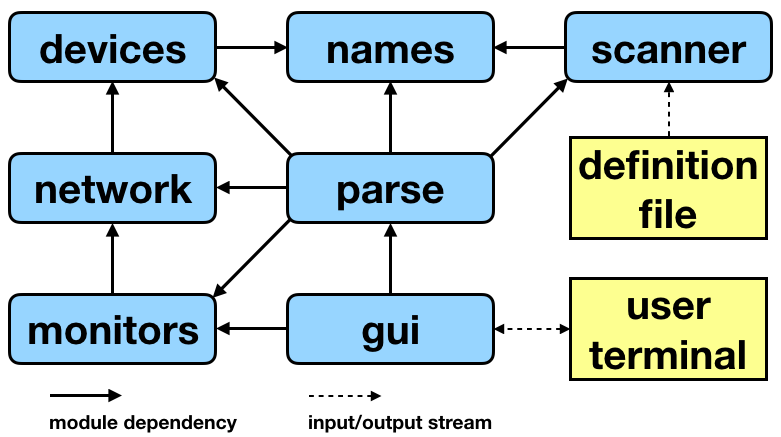
\includegraphics[width=0.8\textwidth]{./figures/dependency.png}
\caption{\label{fig:orgaec3f5b}
Software Structure of the Logic Simulator}
\end{figure}

Figure \ref{fig:orgaec3f5b} illustrates the software structure of the logic
simulator, which shows the module names and their dependencies. The
dependency profile shown in figure \ref{fig:orgaec3f5b} is not the whole
story: it only shows \emph{major} dependencies in order to make the diagram
more clean and intuitive (actually in the source code \texttt{gui.py} depends
on all other modules, but it's tedious and unnecessary to draw them
all). The following subsections will explain the modules in turn.

\subsection{The \texttt{names} module}
\label{sec:orgb27eba3}

The \texttt{names} module is the simplest one among all the modules, but it's
a crucial part of the simulator since all the other modules depend on
it, either directly or indirectly. The main function of the \texttt{names}
module is to assign each name string (can be device name, keywords,
etc.) a unique id (a non-negative integer), so that other modules can
communitate with each other through the ids instead of using the
actual name strings. The \texttt{names} module can also assign unique error
codes to the error-name lists of the other modules, which is very
useful in the error-handling stage. 

\subsection{The \texttt{devices}, \texttt{network} and \texttt{monitors} modules}
\label{sec:org0a9238d}

The three modules \texttt{devices}, \texttt{network} and \texttt{monitors} together store
almost all the information of the circuit configurations.

The \texttt{devices} module stores all the individual devices used in the
logic circuit. This module depends on the \texttt{names} module and use the
allocated ids from \texttt{names} to identify the devices. Each stored device
has a unique device id, a device type, input port connections, output
port values and additional device settings. In general, the \texttt{devices}
module is mainly used to create new devices and return relevant
information of the stored devices on request.

The \texttt{network} module depends on the \texttt{devices} module. It stores all
the connections among the devices and updates the input/output
signals for new simulation cycles. For each device type, the module
has a method to update the outputs of devices of that type based on
the inputs. The main function of the \texttt{network} module is to establish
new connections among the devices and execute the whole network to
update the signals and move on to the next simulation cycle.

The \texttt{monitors} module depends on both the \texttt{devices} module and the
\texttt{network} module. This module manages the creation and deletion of the
monitors, and it also records the output values of the monitored
signals against time (simulation cycles). Every time after executing
the whole network, the \texttt{monitors} module records the updated output
values for the existing monitors for the new simulation cycle. The
main function of this module is to manage monitors and provide data
for drawing waveforms on the canvas.

\subsection{The \texttt{scanner} and \texttt{parse} modules}
\label{sec:org69f2c8b}

The two modules \texttt{scanner} and \texttt{parse} are at the heart of definition
file read-in and error reporting. In our design, \texttt{scanner} just
converts the definition file to symbols (or tokens), and \texttt{parse}
receive the symbols from \texttt{scanner} and construct the circuit network.
The \texttt{parse} module also does all the error handling.

The \texttt{scanner} module reads the definition file directly and converts
the file to a series of symbols. A symbol is a low-level abstraction
of the input file stream, which can be a \texttt{KEYWORD}, a \texttt{NAME}, a
\texttt{NUMBER}, a \texttt{PUNCTUATION} or the \texttt{EOF} (end of file) token. In our
design, the scanner does not do any error handling, but there are
circumstances where the current symbol cannot be categorised to any of
the types stated above. Examples are number with leading zeros (\texttt{007})
and unrecognised characters (\texttt{?!@\#\$}). Therefore, apart from the
normal types stated above, we have included a new type \texttt{SYNTAX\_ERROR}
to deal with this case.

The \texttt{parse} module takes as input the symbols from \texttt{scanner} and builds
the circuit network on the fly. The \texttt{parse} module tries to interpret
the symbol stream as statements explained in Section \ref{orgb2fd366},
and then call methods in \texttt{devices}, \texttt{network} and \texttt{monitors} to create
new devices, connect device ports and add new monitors. If it detects
an error, it will generate an error code, display the description and
location of the error and seek the next left parenthesis \texttt{'('} to
resume parsing. User cannot proceed to the simulation stage if \texttt{parse}
generates errors.

\subsection{The \texttt{gui} module}
\label{sec:org7fd0f3f}

The \texttt{gui} module implements the graphical user interface for the logic
simulator to interact with the user directly. Technically the \texttt{gui}
module has dependencies on all other modules, but only two major ones
are drawn in figure \ref{fig:orgaec3f5b} to make the diagram clean and
intuitive. When the user launches the simulator, \texttt{gui} first calls the
\texttt{parse} module to read the selected definition file, and then use the
data in the \texttt{monitors} module to add/delete monitors and draw the
signal waveforms on the canvas. \texttt{gui} also calls the \texttt{network} module
to move to next simulation cycle, and calls \texttt{devices} to alter the
states of the switches.

\section{Teamwork}
\label{sec:orgccb520f}

Since this software project is a group project for three people,
teamwork is very important to keep the development progress smooth and
efficient. We have taken several simple but useful approaches to let
ourselves always work as a team. Our team is a great team with
enthusiasm all the time, and the progress and outcomes are quite as
expected.

\subsection{Task allocation among team members}
\label{sec:org1a6ee52}

There are four main modules that need to be implemented by us:
\texttt{names}, \texttt{scanner}, \texttt{parse} and \texttt{gui}. Initially we have split the
work into three parts: \texttt{names} \& \texttt{scanner} (Paul), \texttt{parse} (me) and
\texttt{gui} (Brian). Apart from the dependency relationships among these
modules, they are actually quite independent so that we can start
implementing our modules at the same time. Also, by this arrangement,
we can avoid merge conflicts in Git as much as possible since each
individual module is assigned to one team member only.

Due to the nature of the modules, the \texttt{gui} module needs much more
work than other modules. With efforts, the implementation, integration
and testing of the \texttt{names}, \texttt{scanner} and \texttt{parse} modules were
finished much faster than expected, before the completion of the \texttt{gui}
module. Therefore, me and Paul joined the \texttt{gui} implementation
afterwards, based on the framework set up by Brian. This has led to
more merge conflicts, but with the coordination of \texttt{gui} designer
Brian and frequent group meetings they have been easily resolved.

\subsection{Teamwork on code review}
\label{sec:orgda3e6d5}

Code review is an important measure to keep the whole team
coordinated. It involves detecting hidden bugs, revising the code
style (check PEP8 compliance) and all other methods that can improve
the overall software quality. When we write our own modules, we also
take a look at modules implemented by other team members and give them
short feedbacks as soon as possible. The code review process not only
makes our software more robust, but also helps each team member better
understand other teammates' work.

\subsection{Group meetings}
\label{sec:org6d55e23}

Group meeting is an efficient way to share ideas and make important
decisions within the group. During this project, we have held a lot of
group meetings very frequently, roughly once every 2-3 days (other
than the scheduled DPO sessions). By having frequent group meetings,
we can summarise the finished work and make new short-term plans and
decisions very rapidly. 

Many key decisions have been made during the group meetings. For
example, the EBNF syntax definition was made in our first two group
meetings, even before the first scheduled DPO session of the project.
Other decisions include the basic framework of each module, and the
desired functions and features in the \texttt{gui} module.

Another important aspect in the group meetings is to specify the
interfaces among modules. The tight dependencies among modules implies
that we have to design the module interfaces very carefully before we
actually implement the methods in each module. For instance, we spent
a whole group meeting designing the interface between \texttt{scanner} and
\texttt{parse}, since we need various features in error handling such as
displaying the line and position of each error occured. The effort on
the interface specification has led to very successful integration of
the \texttt{scanner} and \texttt{parse} module.

\subsection{Compromise within the team}
\label{sec:orga9e018c}

In this project, there are occasions where we have different ideas on
particular aspects of design. This happens a lot in the design and
implementation in the \texttt{gui} module. For example, I once suggested
Brian to enlarge the main control panel and display both the active
monitor list and the switch list on the panel, but Brian wanted to
keep the panel as simple as possible. Finally we figured out a
`compromised version' in which the switch list is embedded in the
panel while the monitor list is acheved by a pop-up window.

Sometimes we also need to compromise on our ambitions since we always
have endless imporvement plans but there are also limitations on
available time and resources. For instance, in the
internationalisation stage of the software, the translation of the
hoverbox has been a big headache since its rendering is handled by
GLUT rather than the operating system, and the GLUT has no internal
support for rendering Unicode characters. In the end, we used a
`hand-crafted' solution: draw the Chinese hoverbox manually, make a
screenshot of it and then render the image on the canvas.




All the classes and methods written by us need to be tested, either
formally or informally. The \texttt{gui} module needs to be tested by
numerous experiments on the actual software, while the other modules
can be tested formally using the \texttt{pytest} module.


\section{My Contribution to the Project}
\label{sec:org57dc4e1}

As stated in the previous section, I am in charge of the design,
implementation and testing of the \texttt{parse} module, while actually I
have also contributed to some parts of the \texttt{gui} module. The following
subsections will explain the details of my contribution.

\subsection{\texttt{parse.py}}
\label{sec:orgdb599ed}

This module is used to parse the definition file and build the logic
circuit network. It analyses the syntactic and semantic correctness of
the symbol stream from \texttt{scanner} and displays a collection of error
messages if errors occur.

\subsubsection{Basic elements}
\label{sec:org19573e6}

The variables \texttt{self.symbol\_type} and \texttt{self.symbol\_id} are used to
store the information of the current symbol, received from the
\texttt{scanner}. \texttt{self.symbol\_type} can be one of the following:
\texttt{self.scanner.KEYWORD}, \texttt{self.scanner.NAME}, \texttt{self.scanner.NUMBER},
\texttt{self.scanner.PUNCTUATION}, \texttt{self.scanner.SYNTAX\_ERROR} and
\texttt{self.scanner.EOF}. \texttt{self.symbol\_id} stores the id of the symbol
content which can be used in the \texttt{names} module to find the actual
name string (for the \texttt{NUMBER} type, the id is the number itself). The
method \texttt{self.move\_to\_next\_symbol()} is used to get next symbol from
scanner and update the \texttt{self.symbol\_type} and \texttt{self.symbol\_id}.

The \texttt{parse} module has defined 32 error types whose error codes are
assigned by the \texttt{names} module's method
\texttt{self.names.unique\_error\_codes(32)}. The dictionary \texttt{self.errormsg}
maps an error code to its corresponding error message, which forms the
basis of error message display. An important variable,
\texttt{self.error\_code}, is used to store the current error code. When error
occurs during parsing, \texttt{self.error\_code} will be modified and the
parser will call \texttt{self.error\_display()} to display the error message
based on the error code in \texttt{self.error\_code}.

\subsubsection{Mechanism of parsing and error handling}
\label{sec:org08be7c5}

The logic of parsing definition files is simple: each non-terminal
variable is represented by a method in \texttt{parse.py}, and the method
returns \texttt{True} or \texttt{False} to indicate whether the symbols can be
interpreted as that non-terminal variable in the EBNF syntax.

The parsing process is initiated by calling \texttt{self.parse\_network()},
which tries to read the entire definition file and build the circuit
network. \texttt{self.parse\_network()} calls \texttt{self.statement()} repeatedly to
read the statements in the file, and \texttt{self.statement()} calls
lower-level methods like \texttt{self.device()}, \texttt{self.connect()} and
\texttt{self.network()} and the recursive process continues according to the
EBNF syntax. 

If error occurs in a parser method, it stores the corresponding error
code into \texttt{self.error\_code} and return \texttt{False}. Then, the parsing
process will eventually get back to the root method
\texttt{self.parse\_network()} and the method \texttt{self.error\_display()} will be
called to produce the relevant error message. In addition, it's
interesting to notice that if a method detects an error it will
definitely return \texttt{False}, but if a method returns \texttt{False} it does not
necessarily mean an error has occured - it might just mean the current
symbol cannot be interpreted as the non-terminal variable represented
by that method, and it's harmless.

\subsubsection{Main features of error display}
\label{sec:orgf7b2cbd}

The \texttt{self.error\_display()} has many useful features which help the
user locate and correct the errors more easily. This subsection lists
these features and briefly introduces the mechanisms behind the scene.

\begin{enumerate}
\item Display of the error location
\label{sec:org6e3d71d}

For each error, the error message shows the content of the line in
which the error occurs, together with its line number and the position
of error in that line. This is achieved with the help of \texttt{scanner}'s
method \texttt{self.scanner.complete\_current\_line()}, which returns the
current line content and the position of the current symbol. The line
number can be obtained by \texttt{self.scanner.line\_number}. 

\item Additional information in error description
\label{sec:org38081ff}

The error description for the error \texttt{self.DEVICE\_REDEFINED} is:

\texttt{"***Semantic Error: Device '\{symbol\_name\}' is already defined"}

Notice the curly brace pattern \texttt{\{symbol\_name\}} - it's a placeholder
for the actual name of the current symbol. For example, if the current
symbol name is \texttt{'D1'} (which represents a device name), the
placeholder \texttt{\{symbol\_name\}} will be replaced by \texttt{D1}. Internally, this
is done by using \texttt{str.format(**format\_dict)}, where \texttt{format\_dict} is
\texttt{self.errormsg.format\_dict} in my implementation. The \texttt{format\_dict} is
a dictionary which maps keyword such as \texttt{symbol\_name} to its actual
name string. 

The curly brace placeholders also exists in error descriptions of
other error types. This feature provides additional information to the
user which helps the user better understand his/her error.

\item Display of the line of previous definition
\label{sec:org24a5586}

If the user redefines a device or monitor, the line of previous
definition will also be shown, together with the error message of
current line. This is achieved by recording the line number and
position of each device/monitor definition in two dictionaries (one
for device and one for monitor). The \texttt{scanner} module has a list
called \texttt{self.scanner.previous\_lines} where content of previous lines
can be obtained. With this list and the two dictionaries, the line of
previous definition of a device/monitor can be easily displayed.

\item Device name suggestion system
\label{sec:org29b2a6f}

In the \texttt{CONNECT} and \texttt{MONITOR} statements, if a device name cannot be
recognised (not defined), a suggestion list of possible existing
device names will be displayed together with the error message. The
suggestion algorithm is based on the maximum length of the common
prefix of two strings. For example, if the existing device list is
\texttt{[A1 B11 B12 B2 C3]} and a user types \texttt{B1}, the suggestions would be
\texttt{[B11 B12]}.
\end{enumerate}

\subsection{\texttt{test\_parse.py}}
\label{sec:orgecf216b}

The \texttt{test\_parse.py} contains the formal testing functions for
\texttt{parse.py}, which includes unit tests and integration tests. Unit
tests are used to test the individual methods, while integration tests
are used to test the functionality of the whole module. Brian wrote
the unit tests to test each method and I wrote the integration tests
to test whether the parser is able to generate correct error codes
when given a test definition file.

To simplify the testing process and avoid creating loads of test files
in the project folder, I have implemented a class called
\texttt{ParserTestCase} to help me do the integration tests. An instance of the
\texttt{ParserTestCase} class reads the definition file input as Python
strings, execute the parser and check if the produced error codes are
the same as expected.

The method \texttt{self.add\_input\_line(line)} adds a line to the test file
where \texttt{line} is a Python string. The method
\texttt{self.add\_expected\_error(name,linum,pos)} appends a 3-tuple (the name,
line number and position of the expected error) to
\texttt{self.expected\_output} which is a list of expected errors. After
constructing a test case using the two methods above, the parser is
executed and the actual produced errors are stored in
\texttt{self.actual\_output}. Finally the actual output is compared to the
expected output to decide whether the test case is passed.

I have written test functions for all possible error codes using the
\texttt{ParserTestCase} class, and they all get passed. 

\subsection{\texttt{gui.py}}
\label{sec:org8a7a4c1}

My main contribution to \texttt{gui.py} is the implementation of the yellow
hoverbox which shows the current cycle number, output port name and
its output value (high/low) when the cursor is placed inside the
canvas. An example of the yellow hoverbox can be found in Appendix C
(the one-page user guide). I have also added a `dragging function' in
\texttt{gui.py}, which allows user to drag the signals up and down to adjust
the vertical order of the signal waveforms.

In the maintenance stage, I also implemented the Chinese version of
the hoverbox. Since the GLUT have no internal support for Unicode
rendering, I used a `hand-crafted' approach instead: draw the hoverbox
on computer, take its screenshot and use texture mapping to display it
on the canvas. This is the best workaround we can find in the limited
project time.

\section{Testing Procedures}
\label{sec:orgd2879f4}

\section{Possible Improvements}
\label{sec:org8314ce4}

\section{Conclusion}
\label{sec:org035f984}
\end{document}